\documentclass[12pt]{IEEEtran}
\IEEEoverridecommandlockouts

\usepackage{cite}
\usepackage{amsmath,amssymb,amsfonts}
\usepackage{graphicx}
\usepackage{textcomp}
\usepackage{xcolor}
\usepackage{booktabs}
\usepackage{tabularx}
\usepackage{multirow}
\usepackage{makecell}
\usepackage[hypertexnames=false]{hyperref}
\usepackage{microtype}
\usepackage{array}
\usepackage{float}

\hbadness=10000
\vbadness=10000
\hfuzz=20pt
\vfuzz=20pt
\emergencystretch=2em

\def\BibTeX{{\rm B\kern-.05em{\sc i\kern-.025em b}\kern-.08em
    T\kern-.1667em\lower.7ex\hbox{E}\kern-.125emX}}

\begin{document}

\begin{titlepage}
\centering
\vspace*{\fill}

{\Large \textbf{Title:}\\
\textbf {ATELIER: A Hybrid Neuro-Symbolic Multi-Agent Framework for Predicting Public Sentiment Dynamics, Emotional Contagion, and Backlash in Digital Ecosystems} \par}

\vspace*{\fill}

{\Large \textbf{Applicant:}\\
SVKM DWARKADAS J SANGHVI COLLEGE OF ENGINEERING\par}

\vspace*{\fill}

{\Large \textbf{Name of Authors:}\\
Deepali Patil \\
Darshan Jain \\
Atharva Nagarsekar \\
Atharva Patkar \\
Vinayak Mestry \\
Aryan More \par}

\vspace*{\fill}
\end{titlepage}

\title{ATELIER: A Hybrid Neuro-Symbolic Multi-Agent Framework for Predicting Public Sentiment Dynamics, Emotional Contagion, and Backlash in Digital Ecosystems}

\author{\IEEEauthorblockN{Darshan Jain, Atharva Nagarsekar, Atharva Patkar, \\
Vinayak Mestry, Aryan More, and Deepali Patil}

\IEEEauthorblockA{\textit{Department of Artificial Intelligence and Data Science} \\
\textit{SVKM's Dwarkadas J. Sanghvi College of Engineering}\\
Mumbai, India \\
\{jaindarshan1005, nagarsekaratharva, atharva0604, vmestry351, aryansmore167, kolhedeepali20\}@gmail.com}
}

\maketitle

\begin{abstract}
Public opinion cannot be reduced to a single sentiment value that applies to some text. Instead, it arises from an individual's social position, their personality, memory, the structure of their local network, and the dynamics of the online platform. We introduce ATELIER, a neuro-symbolic hybrid model that aims to disentangle the interpretation of an event from the overall reaction of its public. The current model architecture uses an LLM-driven perceptual layer to encode an event into two 12-dimensional tensors representing official and skeptical world states, an urgency score, a relevance marker for the user, bias labels, and a backlash probability. It then uses a deterministic tensor pipeline to propagate the representation through an artificial society that incorporates correlated Big Five personality traits, economic inequality, influential people, sparse graph structure, memory, attentional gating, and collective-action thresholds.

Our research explicitly grounds itself on what the implementation is doing. The current version of ATELIER models distortion of signals by the platform, social consensus perception, relative deprivation, selective exposure, stress induced cognitive tunneling, memory reinforcement, virality, social media polarization, Granovetter-like cascading behaviors, endogenously generated events, and A/B testing on narratives. In controlled evaluation conditions, matched pairs of sentiments exhibit closer behavior to that of a transformer based baseline than unmatched ones; greater event magnitude results in monotonically increasing engagement and collective action; triadic closure leads to greater network clustering; the presence of bridge nodes results in wider cascade propagation; and algorithmic amplification leads to more engagement, and changes the event representation. One should interpret these results as scenarios specific internal validation of ATELIER's performance, but not absolute predictions of real world.
\end{abstract}

\begin{IEEEkeywords}
Agent-based modeling, neuro-symbolic systems, sentiment simulation, polarization, algorithmic amplification, social physics, explainable AI.
\end{IEEEkeywords}

\section{Introduction}
\label{sec:introduction}

Most of the prevalent sentiment analysis approaches solve a limited task that might be insufficiently relevant for addressing more general aims of this research. Namely, they try to determine the sentiment that the text in question has. Even though it might be done with a very good level of accuracy, one would wonder about a slightly more complex and interesting question: What is the reaction of society to the particular event? One might have different reactions to the same news depending on the place occupied within society: joy, fear, anger, indifference, etc.

ATELIER solves this problem by means of a unified pipeline. Initially, the language model builds a world according to the description of the event in question. The next step is feeding the built world into the deterministic PyTorch pipeline which simulates a virtual society made up of various characters distinguished by personalities, possessions, influence, positions within society, memories, and neighbors.

This research does not aim to solve any sociological problems using the computer simulation. Instead, the goal of this paper is to suggest a systems design that relies on mechanics and code. Namely, stress testing is provided for all sorts of entities at once.

\section{System Architecture}
\label{sec:architecture}

\begin{figure*}[t]
\centering
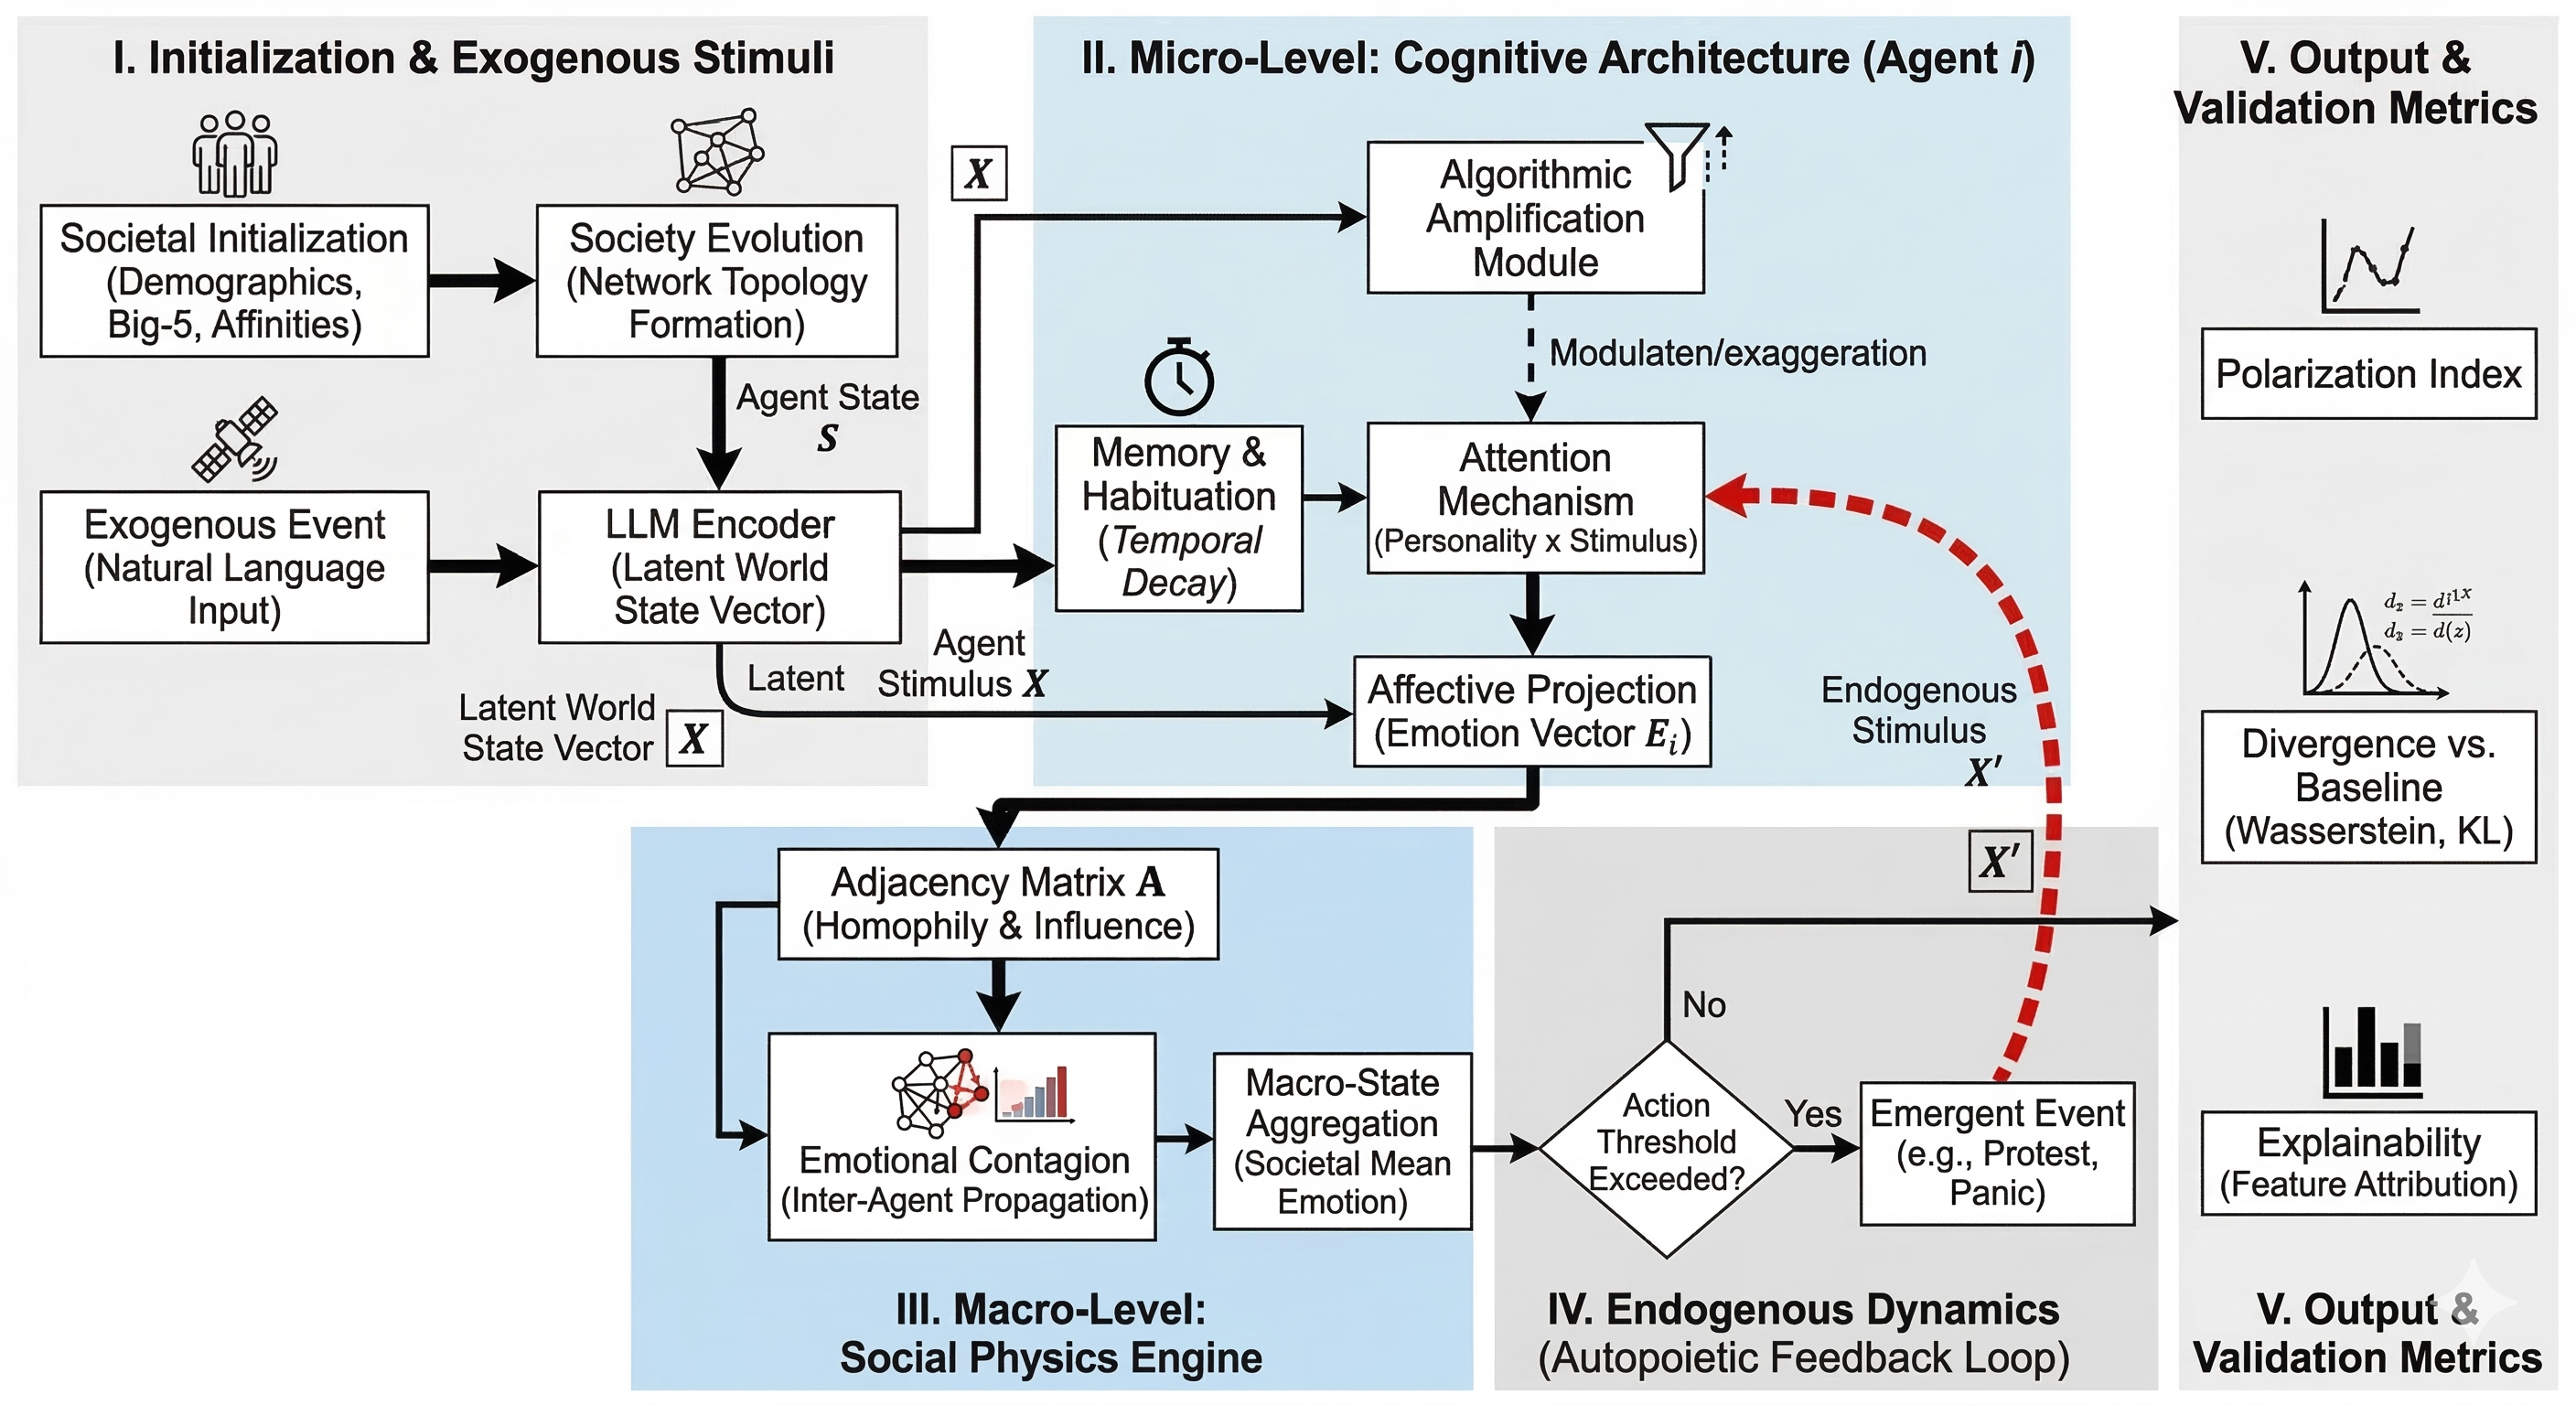
\includegraphics[width=\textwidth]{research_paper_tests/atelier_dataflow.png}
\caption{ATELIER dataflow from event parsing to social aggregation, spanning perception, society generation, cognitive processing, social aggregation, validation, and orchestration.}
\label{fig:dataflow}
\end{figure*}

ATELIER is implemented as a modular pipeline rather than a single monolithic predictor.

\subsection{Neuro-Symbolic Decomposition}

The framework is hybrid for practical reasons, not as a branding exercise. Driving every agent directly with an LLM would introduce substantial stochasticity, computational cost, and auditing difficulty. ATELIER therefore uses an LLM only in the perception layer, where an event is distilled into a compact symbolic representation consisting of official and skeptical world tensors, urgency, personal relevance, and framing cues. Once that projection is complete, the rest of the pipeline is executed as deterministic tensor algebra over a full synthetic population. This split preserves semantic flexibility at the input boundary while keeping large-scale social simulation fast, reproducible, and interpretable.

\subsection{Explicit Schema}

\begin{table}[H]
\caption{ATELIER's symbolic world schema and emotion basis.}
\label{tab:schema}
\centering
\begin{tabular}{@{}rlrl@{}}
\toprule
\multicolumn{2}{c}{\textbf{World Dimensions}} & \multicolumn{2}{c}{\textbf{Emotion Basis}} \\
\midrule
0 & Wealth & 0 & Joy \\
1 & Physical Safety & 1 & Trust \\
2 & Stability & 2 & Fear \\
3 & Reputation & 3 & Surprise \\
4 & Fairness & 4 & Sadness \\
5 & In Group & 5 & Disgust \\
6 & Innovation & 6 & Anger \\
7 & Freedom & 7 & Anticipation \\
8 & Sanctity &  &  \\
9 & Care &  &  \\
10 & Short Term &  &  \\
11 & Long Term &  &  \\
\bottomrule
\end{tabular}
\end{table}

Each event is represented as a world tensor $\mathbf{w}\in[-1,1]^{12}$. Agent-level cognition produces a context vector $\mathbf{c}_i$, which is projected into an 8-emotion distribution by
\begin{equation}
\mathbf{e}_i = \text{softmax}\left(\frac{\mathbf{c}_i P}{\tau}\right),
\end{equation}
where $P$ is a fixed 12-to-8 projection matrix and $\tau$ is an emotion-temperature parameter.

\subsection{Attention as Sociology}

One of ATELIER's most distinctive choices is to define attention not over tokens, but over structural exposure, deprivation, threat, and worldview alignment. Let $\mathbf{x}_i$ denote agent $i$'s exposure vector and $\mathbf{w}_i$ the perceived event tensor after distortion and social-consensus blending. The relative-deprivation stage first normalizes exposures,
\begin{equation}
\mathbf{s}_i = \frac{\mathbf{x}_i + 1}{2}, \qquad \mathbf{g}_i = 1 - \mathbf{s}_i, \qquad \mathbf{a}_i = \mathbf{s}_i,
\end{equation}
then defines jealousy and protection biases from personality:
\begin{equation}
J_i = N_i \lambda_j + (1-A_i)\lambda_r,
\end{equation}
\begin{equation}
P_i = C_i \lambda_p + E_i \lambda_s,
\end{equation}
where $N_i, A_i, C_i,$ and $E_i$ denote neuroticism, agreeableness, conscientiousness, and extraversion, respectively. The initial sociological query is then
\begin{equation}
\mathbf{Q}_i^{(0)} = \mathbf{x}_i \odot \text{clip}(\mathbf{g}_i J_i + \mathbf{a}_i P_i,\; 0.1,\; 3.0).
\end{equation}
In plain terms, this formalizes ``attention as status anxiety'': deficits amplify attention through jealousy, while existing assets amplify attention through protection.

Selective exposure then implements a bounded filter-bubble mechanism. Defining normalized worldview and event vectors,
\begin{equation}
\hat{\mathbf{x}}_i = \frac{\mathbf{x}_i}{\|\mathbf{x}_i\|+\epsilon}, \qquad
\hat{\mathbf{w}}_i = \frac{\mathbf{w}_i}{\|\mathbf{w}_i\|+\epsilon},
\end{equation}
their alignment is
\begin{equation}
\alpha_i = \hat{\mathbf{x}}_i \cdot \hat{\mathbf{w}}_i.
\end{equation}
Openness modulates tolerance to contradiction:
\begin{equation}
o_i = \sigma\!\left(g(O_i - 0.45)\right),
\end{equation}
\begin{equation}
\tau_i = \tau_{\text{base}} - (1+\lambda_o)o_i,
\end{equation}
and the suppression gate becomes
\begin{equation}
S_i = s_{\max}\,\sigma\!\left(g(\tau_i-\alpha_i)\right),
\end{equation}
where $g$ is a configured gain parameter. The filtered query is therefore
\begin{equation}
\mathbf{Q}_i^{(1)} = \mathbf{Q}_i^{(0)}(1-S_i).
\end{equation}
Low-openness agents suppress contradictory events more strongly, while high-openness agents retain more of the signal.

After further key processing based on threats, interaction in different dimensions, thermal regulation, and engagement gating, the model produces an agent context vector. The underlying idea here is that the Q–K architecture is not simply being used as a neural analogy but rather re-purposed as a framework for deprivation, confirmation bias, and salience.

\subsection{Projection Priors}

\begin{table}[t]
\caption{Illustrative high-magnitude psychological priors in the fixed projection matrix.}
\label{tab:priors}
\centering
\begin{tabular}{@{}lll@{}}
\toprule
\textbf{World Signal} & \textbf{Emotion} & \textbf{Weight} \\
\midrule
Fairness deficit & Anger & $-0.8$ \\
Physical-safety deficit & Fear & $-0.8$ \\
In-group cohesion & Trust & $+0.8$ \\
Sanctity violation & Disgust & $-0.8$ \\
Innovation increase & Surprise & $+0.6$ \\
Freedom increase & Joy & $+0.6$ \\
\bottomrule
\end{tabular}
\end{table}

These priors are not hidden inside a latent space. Fairness deficits, for example, are mapped strongly to anger, while in-group cohesion is mapped strongly to trust. That makes downstream emotional dynamics easier to inspect, but it also means the framework inherits the assumptions built into its projection matrix.

\subsection{Synthetic Society, Topology, and Temporal Depth}

This society generation stage builds an ongoing synthesis population rather than generating a small number of hand-scribbled archetypes. Inequality in terms of wealth and influence exists by design; while topology emerges via processes like homophily, bridge creation, and triadic closure. For instance, for a typical society comprising of 10,000 individuals, the process yielded a highly skewed society characterized by the presence of approximately 5.6\% elite individuals, 44.2\% middle class individuals, and 26.6\% working class individuals. The simulation yielded baseline wealth Gini of close to 0.20; maximum influence of well over 300; and a sparsely connected graph with approximately two million non-zero edges.

ATELIER also takes temporal considerations further from one single cycle to more cycles. Evolution involves the processes of inheritance (with redistribution), reinvestment, shocks, mobility, and ideological drift. Briefly, wealth dynamics follow the process of inheritance $\rho W_i^{(t)}$, a redistributed total tax pool $T^{(t)}$, and noisy returns $\xi_i^{(t)}$, while non-wealth exposures drift toward or away from a social attractor:
\begin{equation}
W_i^{(t+1)} = \rho W_i^{(t)} + \frac{T^{(t)}}{N} + \xi_i^{(t)},
\end{equation}
\begin{equation}
\mathbf{x}_i^{(t+1)} = \tanh\!\left(\mathbf{x}_i^{(t)} + \beta_t(\boldsymbol{\mu}^{(t)}-\mathbf{x}_i^{(t)}) + \eta_i^{(t)}\right),
\end{equation}
with optional repulsion for alienated agents. This makes the simulator suitable not only for immediate event diffusion but also for multi-generation structural change.

\subsection{Social Physics, Cascades, and Autopoiesis}

The social-aggregation stage combines agent-level emotion into objective, viral, and elite centers. Structural influence is log-saturated and then multiplied by engagement to implement ``skin in the game'' weighting. Polarization is estimated using a bimodality coefficient along the dominant emotional axis:
\begin{equation}
BC = \frac{\text{Skew}^2 + 1}{\text{Kurtosis} + \epsilon}.
\end{equation}

Collective action follows a Granovetter-style threshold mechanism. Let $\ell_i$ denote the local emotional center around agent $i$. Social validation is
\begin{equation}
V_i = 1 + \cos(\mathbf{e}_i,\ell_i),
\end{equation}
and the individual cost of action is
\begin{equation}
\text{Cost}_i = c_0 - 0.1E_i - 0.1N_i - 0.05\log(1+\text{Influence}_i),
\end{equation}
where $c_0$ is a configurable base action cost, clamped below by a minimum positive floor. Internal motivation is then
\begin{equation}
M_i = \|\mathbf{e}_i\|_2 \, V_i - \text{Cost}_i.
\end{equation}
If topology-aware thresholds are enabled, each agent also carries a personal following threshold
\begin{equation}
\theta_i = \text{clip}\!\left(\mu_G + (C_i + A_i - 1)\sigma_G,\; 0.01,\; 0.9\right),
\end{equation}
becoming active if there is emotional salience, engagement, and either intrinsic motivation or enough local activation. So, the graph is meaningful, because local acting ratios become part of the activation process.

Finally, ATELIER is autopoietic only within the confines that it can create new events from instability in macro levels. When the acting ratio surpasses the configured threshold for action, when elite divergence surpasses its threshold, when polarization is high and valence is lower than about $-0.2$, the simulator outputs a \emph{Populist Uprising} event. When there is high polarization, negative valence, and the predominant emotional contagion has stabilized at anger, disgust or sadness, the framework will output a \emph{Civil Protest}. In summary, the theoretical framework can create a positive feedback effect where society responds to the event, creates instability, and creates new events from within.

\section{Experimental Protocol}
\label{sec:protocol}
This evaluation, presented in this paper, is based on controlled scenario-based research harnesses instead of anecdotal case studies. The harnesses include semantic alignment, sentiment mapping, response limits, low salience filtering, bridge diffusion, inequalities, topology, memory replay, algorithmic amplification, virality limits, demographic segmentation, endogenous occurrences, and backlash A/B testing routes.

These headline figures above are extracted from the controlled scenarios. Hence, the validation strategy is mostly:

\begin{enumerate}
    \item mechanism verification under controlled conditions,
    \item quantitative summary metrics across those conditions, and
    \item figure-backed interpretation of the resulting behaviors.
\end{enumerate}

This is entirely suitable for a system report, but it does not equate to large-scale validation from empirical population data. The values provided are highly dependent on the seed, event design, and parameters used, and therefore must be viewed as scenario-based results. We will revisit this point in Section\ref{sec:limitations}.

\section{Results}
\label{sec:results}

\subsection{Semantic Alignment}

The system compares its aggregated sentiment distribution with a transformer-based sentiment baseline. In the reported scenario set, the positive-world match distance is 0.2937, compared with a positive-world mismatch of 1.3063, while the negative-world match distance is 0.4356, compared with a negative-world mismatch of 1.1644. Aggregated across these scenarios, the matched Wasserstein distance is 0.5465 and the mismatched distance is 1.1535, yielding a separation gap of 0.6070.

\begin{figure}[t]
\centering
\includegraphics[width=\columnwidth]{research_paper_tests/generated/summary_panels/12_semantic_sentiment.png}
\caption{Semantic-alignment summary used in the paper-values report. Matched conditions are substantially closer than mismatched ones, indicating that the symbolic-cognitive pipeline preserves broad semantic direction.}
\label{fig:semantic}
\end{figure}

This result supports internal semantic consistency rather than direct sociological forecasting accuracy, because the comparison baseline is itself a text classifier rather than observed social behavior.

\subsection{Response Boundaries}

\begin{table}[t]
\caption{Response-boundary results from the generated paper-values report.}
\label{tab:boundaries}
\centering
\begin{tabular}{@{}rrrr@{}}
\toprule
\textbf{Magnitude} & \textbf{Mean Engagement} & \textbf{Acting Ratio} & \textbf{Valence} \\
\midrule
0.0000 & 0.0000 & 0.0000 & 0.0000 \\
0.1500 & 0.1064 & 0.7773 & -0.1100 \\
0.3000 & 0.2311 & 0.8477 & -0.2040 \\
0.4500 & 0.3279 & 0.8828 & -0.2800 \\
0.6000 & 0.4015 & 0.8984 & -0.3390 \\
0.7500 & 0.4581 & 0.9219 & -0.3840 \\
0.9000 & 0.5024 & 0.9258 & -0.4200 \\
\bottomrule
\end{tabular}
\end{table}

This is completely valid in terms of a system report, though it does not represent a broad validation in a population empirical sense. The values are very much dependent on the particular seed, event, and parameters involved and thus can only be considered scenario-specific findings. We will come back to this point in Section

\begin{figure*}[t]
\centering
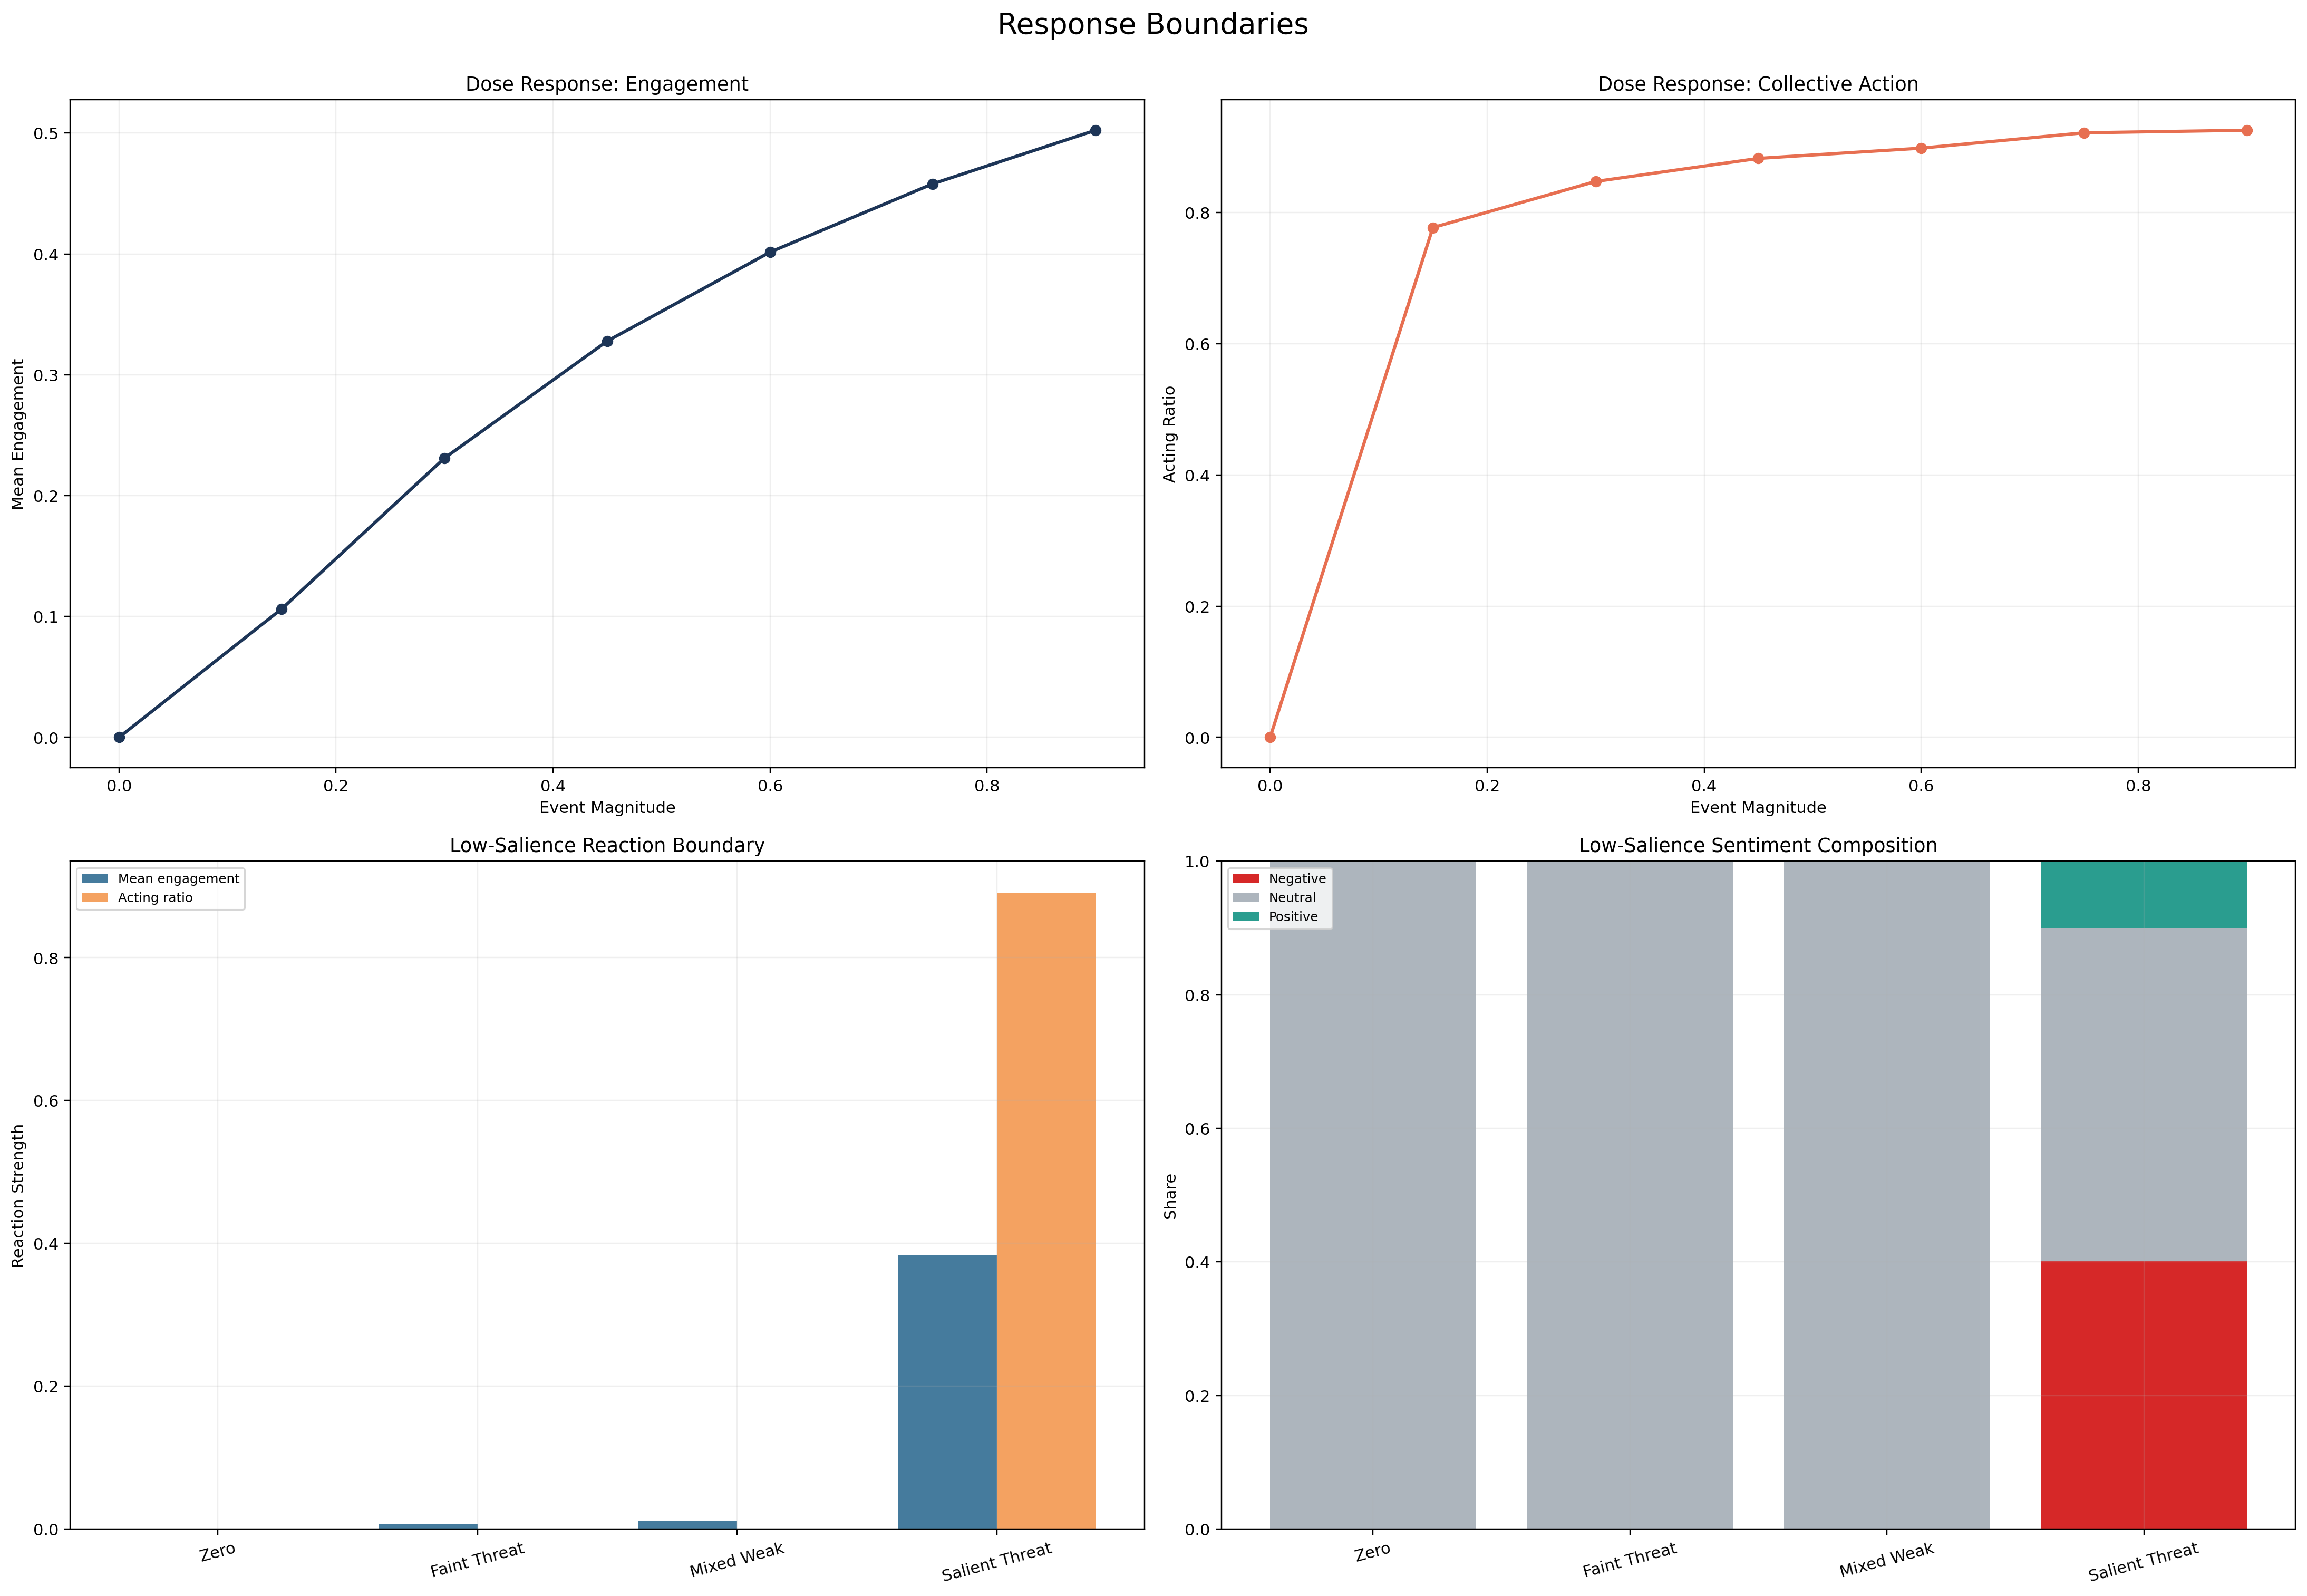
\includegraphics[width=\textwidth]{research_paper_tests/generated/response_boundaries.png}
\caption{Response-boundary results. Top: dose response in engagement and collective action. Bottom: low-salience worlds remain bounded until a sufficiently strong threat is introduced.}
\label{fig:boundaries}
\end{figure*}

\subsection{Population Segmentation}

A central result is the population-segmentation sweep, which varies each world dimension across increasing magnitudes and measures mean engagement for the five structural classes.

\begin{figure*}[t]
\centering
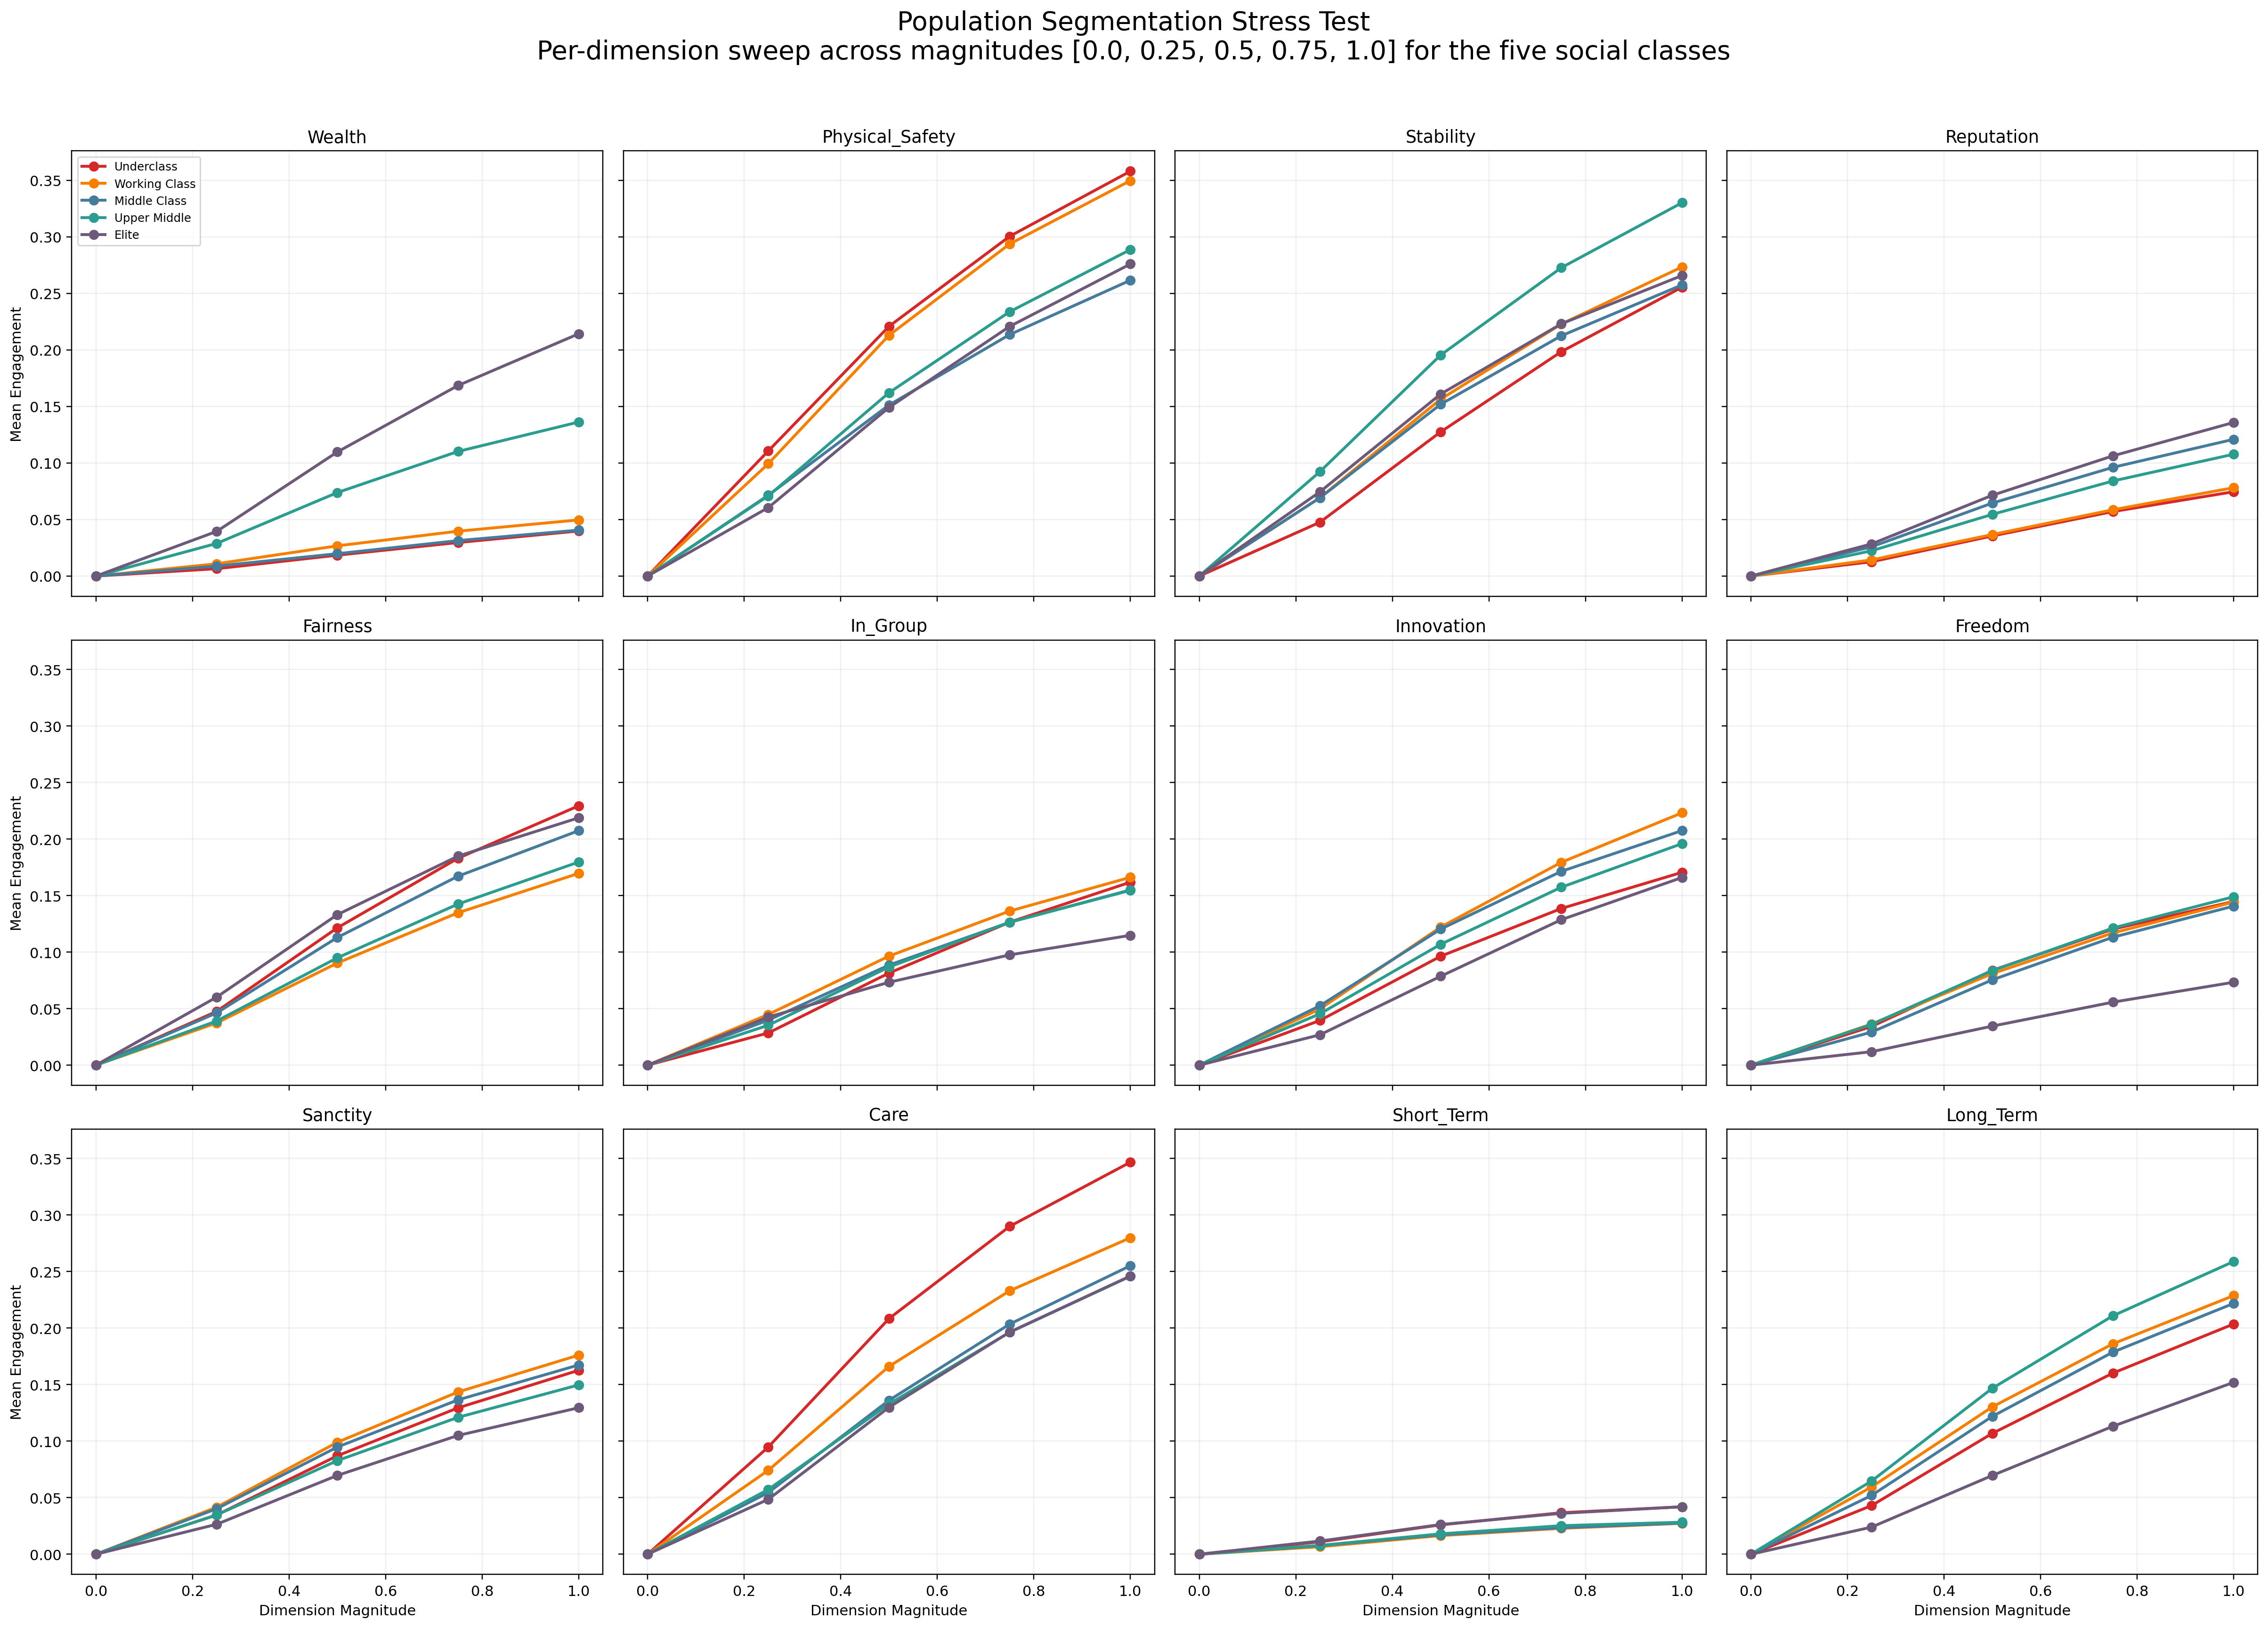
\includegraphics[width=\textwidth]{research_paper_tests/generated/population_segmentation.png}
\caption{Population segmentation stress test. The same world-dimension sweep produces meaningfully different engagement trajectories across classes, especially for Wealth, Physical Safety, Fairness, Care, and Long Term.}
\label{fig:segmentation}
\end{figure*}

Several patterns are clear in Fig. \ref{fig:segmentation}. Upper strata react more strongly to Wealth, Reputation, and Long Term signals. Lower strata react more strongly to Physical Safety, Fairness, and Care. Short Term remains comparatively flat across all classes. The associated experiment also shows that class gaps widen as dimension magnitude increases in the tested setup. This supports ATELIER's core claim that a single event does not need to produce a uniform population response.

\subsection{Inequality, Topology, and Diffusion}

The topology and inequality experiments provide some of the strongest internal evidence in the paper. The reported scenario values are:

\begin{itemize}
    \item baseline wealth Gini: 0.1991,
    \item evolved wealth Gini: 0.3236,
    \item triadic-closure clustering gain: 0.5504,
    \item modularity gain under higher homophily: 0.1853.
\end{itemize}

The bridge-diffusion result is especially informative. In the reported bridge scenario, acting ratio rises from 0.6000 without a bridge to 1.0000 with a bridge, while local arousal in the second community increases by 0.0680. This suggests that the model is sensitive to graph geometry, not only to node attributes.

\subsection{Memory, Amplification, and Virality}

\begin{table}[t]
\caption{Repository-backed metrics for memory, amplification, and virality.}
\label{tab:viralitymetrics}
\centering
\begin{tabular}{@{}lr@{}}
\toprule
\textbf{Metric} & \textbf{Value} \\
\midrule
Memory final norm gain from rehearsal & 5.5924 \\
Algorithmic amplification engagement gain & 0.0444 \\
Algorithmic amplification max world shift & 0.1000 \\
Configured viral cap & 11.0000 \\
Peak viral slope & 39.1250 \\
\bottomrule
\end{tabular}
\end{table}

These factors are important because they account for effects related to time and platform that are typically neglected in sentiment analysis models. Memory rehearsal ensures that signals endure. Algorithmic amplification distorts the world a little bit, but enough to push agents over the threshold required for action. The model of virality is deliberately asymmetrical – extreme emotions are possible to reach a given cap on virality.

\begin{figure}[t]
\centering
\includegraphics[width=\columnwidth]{research_paper_tests/generated/summary_panels/20_virality_bounds.png}
\caption{Virality bounds. In consensus scenarios, mean and max outrage multipliers approach the configured cap. In outlier scenarios, extreme agents saturate the cap while mean virality remains lower.}
\label{fig:virality}
\end{figure}

\subsection{Narrative Backlash and Endogenous Events}

Furthermore, there are two additional high-level approaches used in this code that deserve clear explanation.

Firstly, the approach includes backlash A/B tests. Here, the pioneer group is exposed to the official and skeptical frames, the energy of engagement is counted, and then, one of them wins and propagates throughout the rest of the population. These controlled tests confirm the takeover of the skeptical frame and the persistence of the official one.

Secondly, the code allows for endogenous actions in case both the conditions of polarization and emotional configuration become unstable enough. Experiments show that endogenous action occurs only within an unstable society. Currently, these techniques must be considered as internal validations and cannot serve as predictions of protests or crisis scenarios yet.
\section{Discussion}
\label{sec:discussion}

ATELIER is most persuasive when treated as an interpretable research instrument. Its strengths are structural:

\begin{itemize}
    \item it separates semantic parsing from societal simulation,
    \item it exposes explicit mechanisms for attention, memory, topology, and virality,
    \item it supports class-differentiated reaction rather than scalar sentiment, and
    \item it allows controlled counterfactuals over homophily, urgency, amplification, and narrative framing.
\end{itemize}

It is especially convincing how all these factors combine. Together with this, there is evidence that the simulator does not simply output emotion vectors corrupted by noise but reacts intelligibly to various structural properties of the data.

\section{Limitations and Threats to Validity}
\label{sec:limitations}

Several limitations should be acknowledged directly.

\subsection{Fixed Psychological Priors}

The world-to-emotion projection matrix, the personality-query matrix, and the cross-dimension interactions are all fixed. Their transparency is useful, but they also encode hard priors. If those priors are wrong, the downstream simulation will be wrong in a systematic and internally consistent way.

\subsection{LLM Dependence at the Input Boundary}

The simulator becomes deterministic only after the LLM has produced the official and skeptical world tensors. Semantic drift, prompt sensitivity, or framing bias at that input boundary can therefore propagate through the rest of the system.

\subsection{Synthetic-Population Bias}

ATELIER avoids social-media sampling bias by generating a synthetic society. That is helpful, but it does not eliminate bias; it replaces sampling bias with generator bias. The realism of the population still depends on distributional assumptions, thresholds, and handcrafted structural heuristics.

\subsection{Internal Validation Dominates}

Most of the current evidence is internal: monotonicity checks, mechanism tests, and baseline comparisons. The repository does not yet provide broad empirical calibration against measured real-world cascades, protests, or backlash events.

\subsection{Runtime and Parameter Caveats}

The codebase documentation and inspection suggest that some parameters are weakly connected or effectively inactive in practice, and some frontend controls do not map cleanly to the backend runtime. Any rigorous interpretation of the system should keep these caveats in mind.

\section{Conclusion}
\label{sec:conclusion}
ATELIER goes beyond document-level sentiment classification by integrating structured social simulation into sentiment modeling. The fundamental architecture of ATELIER is based on a clear neuro-symbolic distinction, whereby we utilize one pass of language models to determine event semantics and simulate heterogeneous reactions via tensor mechanics thereafter.

Despite being at early stages of development, the framework allows for the demonstration of a methodological contribution that could be of interest to many researchers. Namely, ATELIER provides a mechanism of creating population with unequal class structure and local neighborhoods, differentiating reactions via mechanisms of deprivation, selective exposure, stress, and memory, and producing metrics such as virality, polarization, elites' divergence, and collective action. All this allows us to test scenarios ex-ante without implementing any change in reality. For instance, policymakers would be able to see how their announcement would be interpreted by certain classes in terms of fear/anger, communication specialists would be able to choose the most effective way of framing the upcoming news, while platforms would be able to test amplification rules in advance.

Nevertheless, our next step is external calibration through better empirical benchmarking, more complex scenarios, and stronger parameter estimation. Prior to the calibration process, however, ATELIER offers much to research from an experimental perspective as well.

\end{document}
